\documentclass[]{article}
\usepackage{lmodern}
\usepackage{amssymb,amsmath}
\usepackage{ifxetex,ifluatex}
\usepackage{fixltx2e} % provides \textsubscript
\ifnum 0\ifxetex 1\fi\ifluatex 1\fi=0 % if pdftex
  \usepackage[T1]{fontenc}
  \usepackage[utf8]{inputenc}
\else % if luatex or xelatex
  \ifxetex
    \usepackage{mathspec}
  \else
    \usepackage{fontspec}
  \fi
  \defaultfontfeatures{Ligatures=TeX,Scale=MatchLowercase}
\fi
% use upquote if available, for straight quotes in verbatim environments
\IfFileExists{upquote.sty}{\usepackage{upquote}}{}
% use microtype if available
\IfFileExists{microtype.sty}{%
\usepackage{microtype}
\UseMicrotypeSet[protrusion]{basicmath} % disable protrusion for tt fonts
}{}
\usepackage[margin=1in]{geometry}
\usepackage{hyperref}
\hypersetup{unicode=true,
            pdftitle={Exploring Revision 8 MCMC},
            pdfborder={0 0 0},
            breaklinks=true}
\urlstyle{same}  % don't use monospace font for urls
\usepackage{longtable,booktabs}
\usepackage{graphicx,grffile}
\makeatletter
\def\maxwidth{\ifdim\Gin@nat@width>\linewidth\linewidth\else\Gin@nat@width\fi}
\def\maxheight{\ifdim\Gin@nat@height>\textheight\textheight\else\Gin@nat@height\fi}
\makeatother
% Scale images if necessary, so that they will not overflow the page
% margins by default, and it is still possible to overwrite the defaults
% using explicit options in \includegraphics[width, height, ...]{}
\setkeys{Gin}{width=\maxwidth,height=\maxheight,keepaspectratio}
\IfFileExists{parskip.sty}{%
\usepackage{parskip}
}{% else
\setlength{\parindent}{0pt}
\setlength{\parskip}{6pt plus 2pt minus 1pt}
}
\setlength{\emergencystretch}{3em}  % prevent overfull lines
\providecommand{\tightlist}{%
  \setlength{\itemsep}{0pt}\setlength{\parskip}{0pt}}
\setcounter{secnumdepth}{0}
% Redefines (sub)paragraphs to behave more like sections
\ifx\paragraph\undefined\else
\let\oldparagraph\paragraph
\renewcommand{\paragraph}[1]{\oldparagraph{#1}\mbox{}}
\fi
\ifx\subparagraph\undefined\else
\let\oldsubparagraph\subparagraph
\renewcommand{\subparagraph}[1]{\oldsubparagraph{#1}\mbox{}}
\fi

%%% Use protect on footnotes to avoid problems with footnotes in titles
\let\rmarkdownfootnote\footnote%
\def\footnote{\protect\rmarkdownfootnote}

%%% Change title format to be more compact
\usepackage{titling}

% Create subtitle command for use in maketitle
\newcommand{\subtitle}[1]{
  \posttitle{
    \begin{center}\large#1\end{center}
    }
}

\setlength{\droptitle}{-2em}

  \title{Exploring Revision 8 MCMC}
    \pretitle{\vspace{\droptitle}\centering\huge}
  \posttitle{\par}
    \author{}
    \preauthor{}\postauthor{}
    \date{}
    \predate{}\postdate{}
  

\begin{document}
\maketitle

I ran Revision 8 using \texttt{rstan} MCMC, running separately on each
of the three risk groups.

\begin{verbatim}
## [1] "initializing..."
\end{verbatim}

\subsection{Results}\label{results}

\subsubsection{Diagnostics: Reliablity, representativeness, and
accuracy}\label{diagnostics-reliablity-representativeness-and-accuracy}

Previously I had run the MCMC algorithm multiple times, getting the same
result each time. This confirms that the posterior is representative of
the underlying data. I didn't repeat the reliability test for the final
analysis because there was very, very little difference between
repetitions in earlier tests.

To assess Representativeness for an MCMC algorithm, we need to see
whether chains have converged such that initial randomly-chosen priors
are not related to final values. We can examine the Gelman-Rubin
statistic (Gelman \& Rubin, 1992), also known as the ``potential scale
reduction factor'' or ``shrink factor''. In \(rstan\), this is available
as the statistic \(\widehat{r}\).

\begin{longtable}[]{@{}lrrrrr@{}}
\caption{group= 1 double\_update\_rev8 1 MCMC vars= 931}\tabularnewline
\toprule
& mean & se\_mean & sd & n\_eff & Rhat\tabularnewline
\midrule
\endfirsthead
\toprule
& mean & se\_mean & sd & n\_eff & Rhat\tabularnewline
\midrule
\endhead
group\_mu\_alpha & 0.33 & 0 & 0.05 & 2055.30 & 1.01\tabularnewline
group\_mu\_beta & 0.55 & 0 & 0.05 & 754.39 & 1.01\tabularnewline
group\_rew\_mu\_alpha & 0.38 & 0 & 0.08 & 2537.63 & 1.00\tabularnewline
group\_pun\_mu\_alpha & 0.29 & 0 & 0.07 & 2437.59 & 1.01\tabularnewline
\bottomrule
\end{longtable}

\begin{longtable}[]{@{}lrrrrr@{}}
\caption{group= 2 double\_update\_rev8 1 NA vars= 1199}\tabularnewline
\toprule
& mean & se\_mean & sd & n\_eff & Rhat\tabularnewline
\midrule
\endfirsthead
\toprule
& mean & se\_mean & sd & n\_eff & Rhat\tabularnewline
\midrule
\endhead
group\_mu\_alpha & 0.34 & 0 & 0.05 & 6833.29 & 1\tabularnewline
group\_mu\_beta & 0.73 & 0 & 0.05 & 4741.86 & 1\tabularnewline
group\_rew\_mu\_alpha & 0.30 & 0 & 0.06 & 6511.53 & 1\tabularnewline
group\_pun\_mu\_alpha & 0.38 & 0 & 0.07 & 5993.03 & 1\tabularnewline
\bottomrule
\end{longtable}

\begin{longtable}[]{@{}lrrrrr@{}}
\caption{group= 3 double\_update\_rev8 1 NA vars= 687}\tabularnewline
\toprule
& mean & se\_mean & sd & n\_eff & Rhat\tabularnewline
\midrule
\endfirsthead
\toprule
& mean & se\_mean & sd & n\_eff & Rhat\tabularnewline
\midrule
\endhead
group\_mu\_alpha & 0.26 & 0.00 & 0.05 & 1919.88 & 1.01\tabularnewline
group\_mu\_beta & 0.65 & 0.01 & 0.08 & 188.82 & 1.05\tabularnewline
group\_rew\_mu\_alpha & 0.31 & 0.00 & 0.08 & 659.24 &
1.02\tabularnewline
group\_pun\_mu\_alpha & 0.21 & 0.00 & 0.06 & 2377.73 &
1.01\tabularnewline
\bottomrule
\end{longtable}

Accuracy can be measured by the effective sample size, as described in
the sectio nabove.

For Group 3, specifically for the group beta parameter, the effective
sample size is just 189, indicating poor sampling for that value.
However, for all other values, the Rhat was in the appropriate range.
For all other groups, the Rhat was within the appropriate range for all
variables of interest.

\subsection{Group differences}\label{group-differences}

The basic graphs show that there is substantial overlap in estimated
alpha and beta parameters within each model.

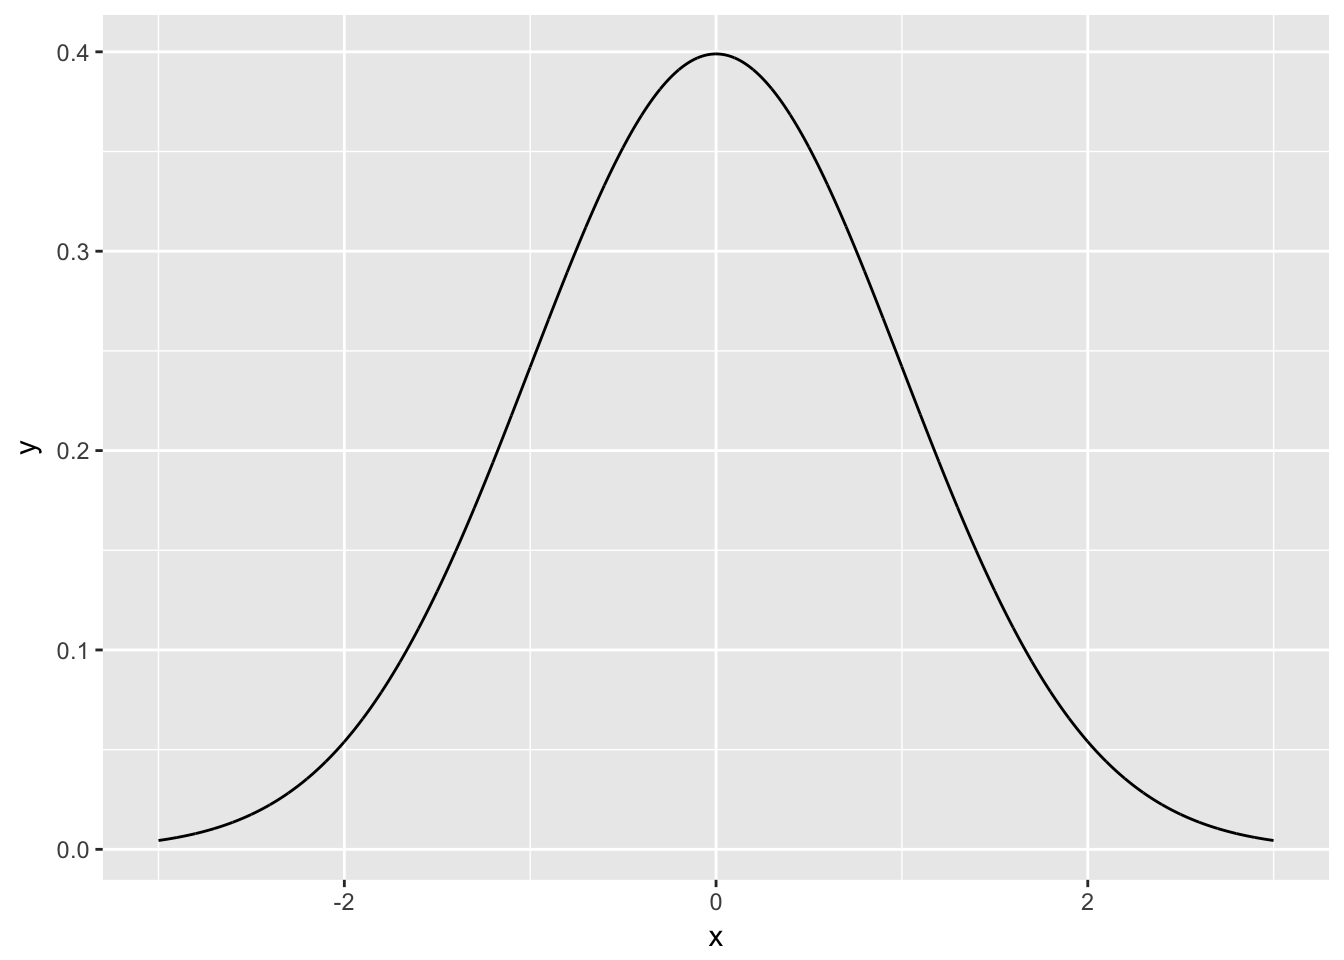
\includegraphics{final_report_three_level_analysis_rev8_files/figure-latex/unnamed-chunk-2-1.pdf}
\includegraphics{final_report_three_level_analysis_rev8_files/figure-latex/unnamed-chunk-2-2.pdf}

\includegraphics{final_report_three_level_analysis_rev8_files/figure-latex/sigma-1.pdf}

We can compare Motivational conditions by subtracting the posteriors
derived for one condition with the posteriors derived in the other
condition.

Comapring reward and punishment estimates, there is not a clear estimate
of a difference of overall performance between the two motivational
conditions.

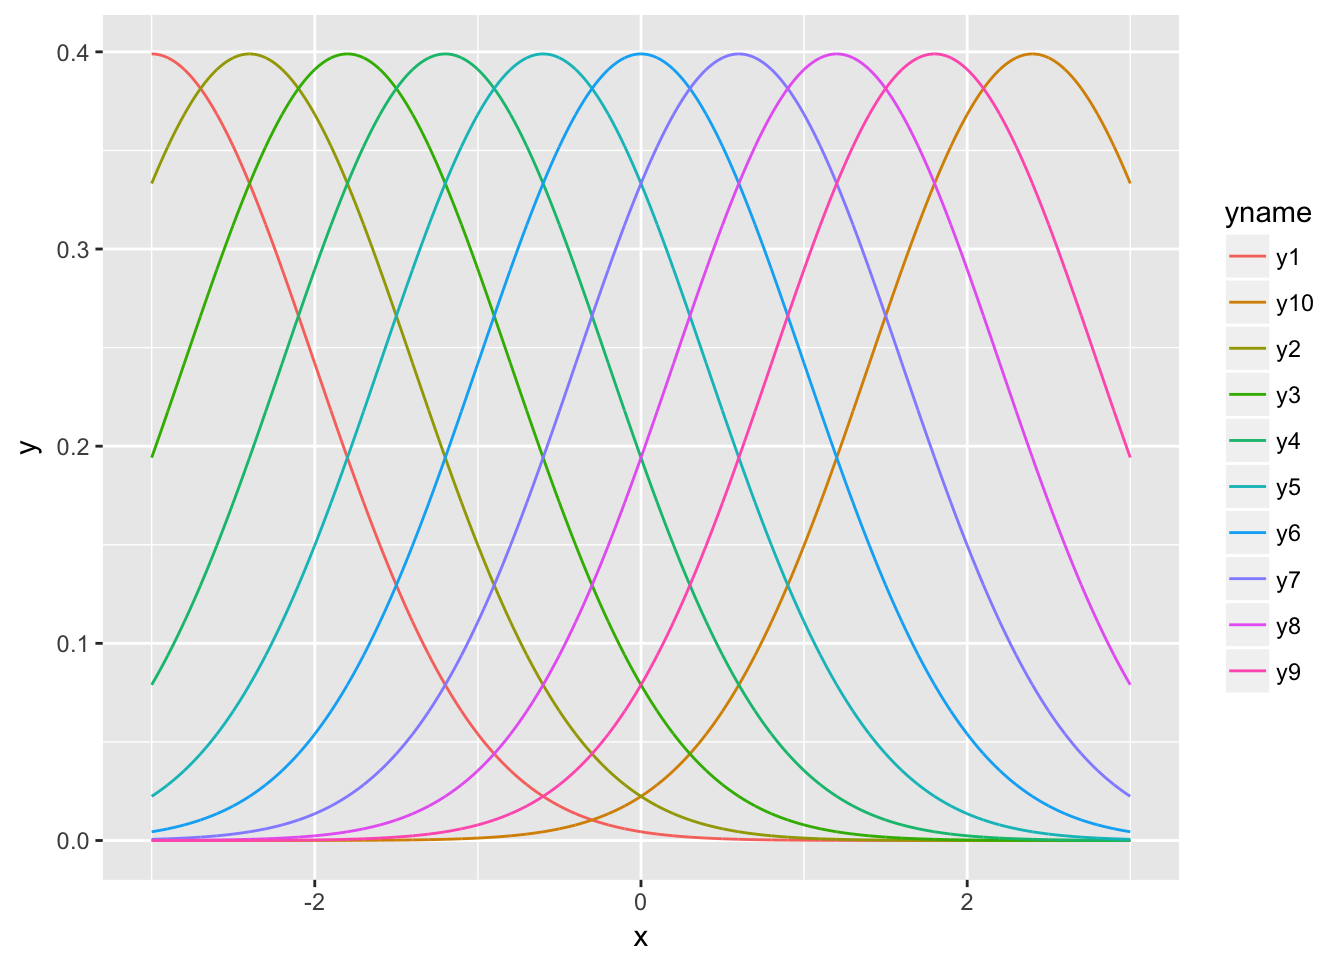
\includegraphics{final_report_three_level_analysis_rev8_files/figure-latex/unnamed-chunk-3-1.pdf}
\includegraphics{final_report_three_level_analysis_rev8_files/figure-latex/unnamed-chunk-3-2.pdf}

We can also compare the groups, looking at group differences overall,
and also specifically at group differences within each reward and
punishment conditions. We use the same method as before: subtracting the
posteriors derived in one group from the posteriors derived in another
group.

In the reward condition, there's no difference apparent in learning rate
between the meth-using group and the other groups. However, in the
punishment condition, there may be some evidence of a difference, with
the Highest Density Interval of the differnce just crossing zero.

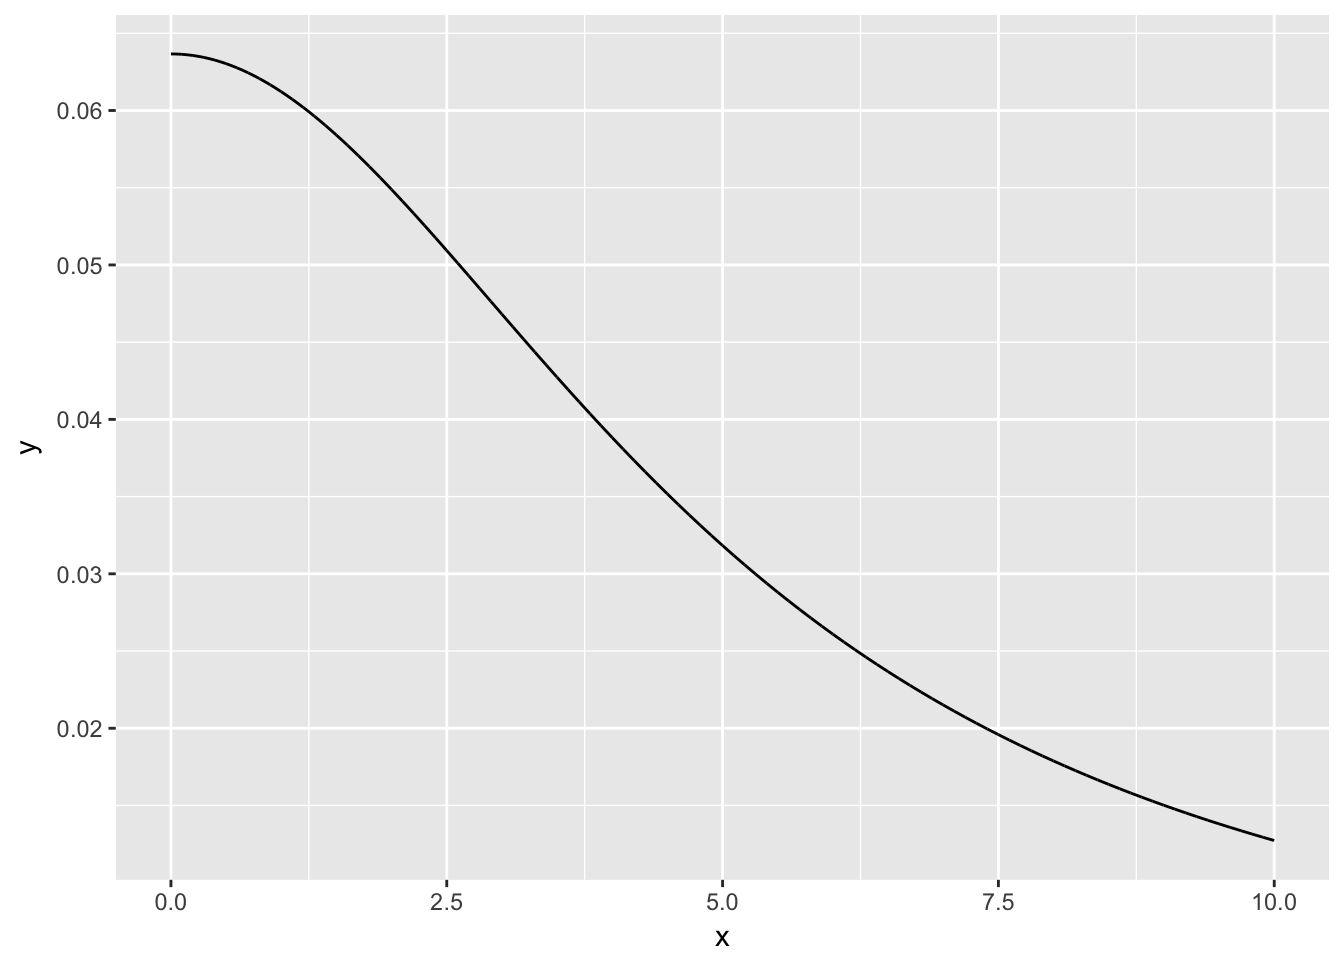
\includegraphics{final_report_three_level_analysis_rev8_files/figure-latex/unnamed-chunk-4-1.pdf}

Comparing group 2 with group 3, there may be a difference between alpha
learning rates in the punishment condition.

\includegraphics{final_report_three_level_analysis_rev8_files/figure-latex/unnamed-chunk-5-1.pdf}

\begin{longtable}[]{@{}lrrl@{}}
\toprule
Statistic & Mean & SD & HDI\tabularnewline
\midrule
\endhead
mu & -0.0848639 & 0.0699501 & {[}-0.22,0.06{]}\tabularnewline
sigma & 0.0220197 & 0.0813884 & {[}-0.13,0.18{]}\tabularnewline
rew\_mu & 0.0126976 & 0.1022954 & {[}-0.18,0.21{]}\tabularnewline
pun\_mu & -0.1761860 & 0.0943302 & {[}-0.37,0.00{]}\tabularnewline
\bottomrule
\end{longtable}

The highest density interval for the difference between Group3 minus
Group 2 still encompassed zero. We can also look at a multivariate 95\%
highest density interval. This uses the R function
\textbar{}MASS::cov.mve\textbar{} to estimate the ellipsoid with the
minimum volume encompassing 95\% of the points.

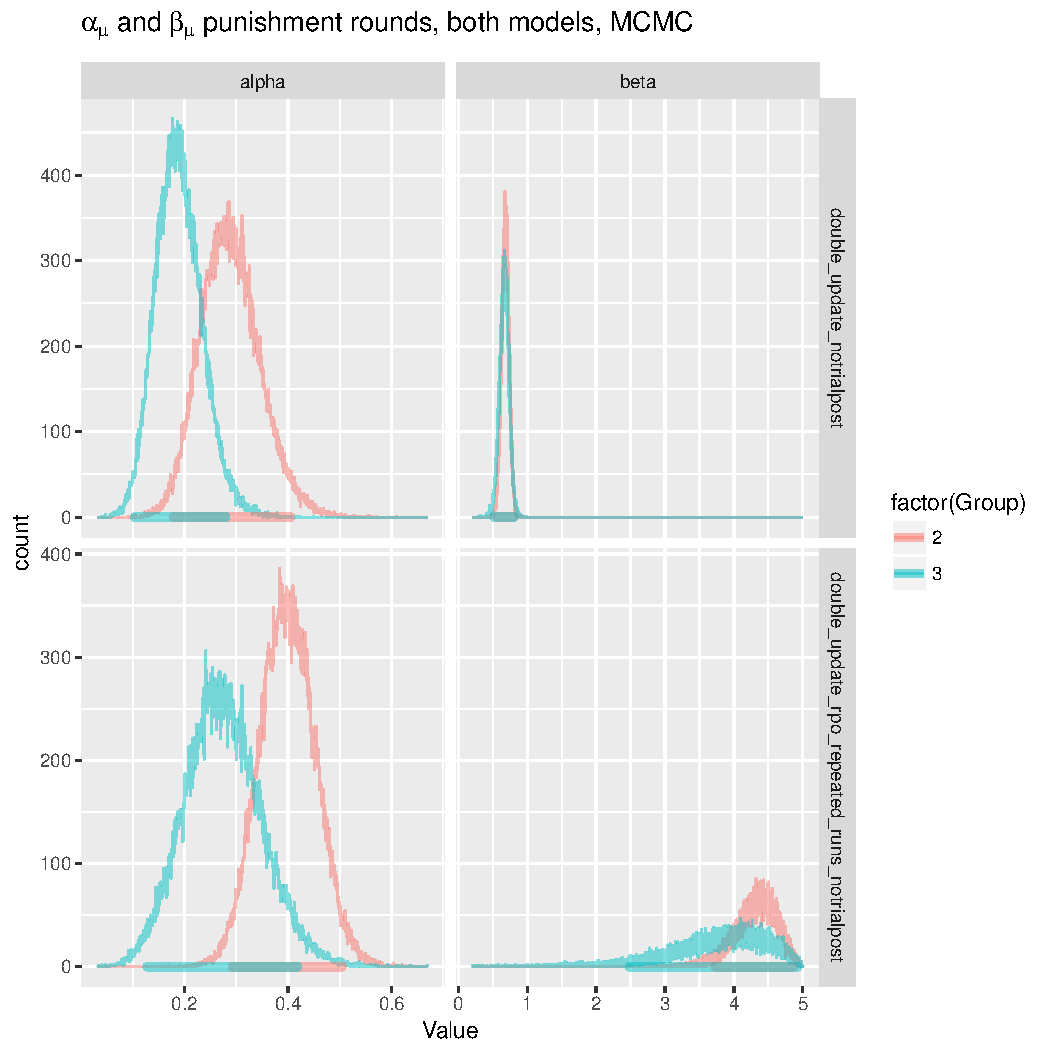
\includegraphics{final_report_three_level_analysis_rev8_files/figure-latex/unnamed-chunk-7-1.pdf}

We can't confirm using a bivariate confidence interval that there is a
difference between the means of Group 2 and Group 3 in the punishment
condition.

\section{Discussion}\label{discussion}

This analysis demonstrates that it is in principle possible to run a
three-level behavioral model in MCMC on our reversal learning dataset. A
joint model built on this initial three-level behavioral model is very
time-intensive to run, and so I have not included it in this thesis.
Still, by examining behavioral data we are able to glean insight into
behavioral patterns. The behavioral model also serves as a useful
baseline for testing the efficacy of joint modeling. It may be that some
insights are available using a joint model that cannot be gleaned using
the method presented here.


\end{document}
